\documentclass{article}

\usepackage[utf8]{inputenc}
\usepackage{pdfpages}
% \usepackage[]{hyperref}
\usepackage{tocloft}

% ---------------------------------------------------------------------------------------
\begin{document}

% ---------------------------------------------------------------------------------------
\begin{titlepage}
    \begin{center}
        \vspace*{1.5cm}
        
        \Huge
        \textbf{{WMC 2022}} \\
        \vspace*{1.5cm}
        
        \large \textbf{Proceedings of the 9th International Workshop on Mixed Criticality Systems} 
        
        \vspace*{2.5cm}
        
        \normalsize
        jointly hold with RTSS 2022, Houston (Hybrid)
        
        \vspace*{4cm}
        
        \large
        \textbf{Edited by} \\
        \vspace*{.2cm}
        \textbf{Xiaotian Dai and Zheng Dong} \\
        \vspace*{.5cm}
        
        
        \vspace*{.5cm}
        December 2022
        
        %\vspace*{1cm}
        %\normalsize
        %All rights reserved by University of York
        
        \vfill
        
    \end{center}
\end{titlepage}

% ---------------------------------------------------------------------------------------
\section*{Organizers}

\noindent \quad

\noindent \textbf{Program Co-chairs}
\vspace{0.5em}

Zheng Dong, Wayne State University

Xiaotian Dai, University of York

\vspace{1em}

\noindent \textbf{Steering Committee}
\vspace{0.5em}

Iain Bate, University of York

Arvind Easwaran, Nanyang Technological University

Zhishan Guo, North Carolina State University

Jing Li, New Jersey Institute of Technology

\vspace{1em}

\noindent \textbf{Program Committee Member}
\vspace{0.5em}

Nan Guan, City University of Hong Kong

Geoffrey Nelissen, Tu Eindhoven

Daniel Casini, Scuola Superiore Sant'anna - Pisa

Lea Schönberger (Publicity Chair), Tu Dortmund University

Kecheng Yang, Texas State University

Konstantinos Bletsas, Cister

Mohamed Hassan, Mcmaster University

Renato Mancuso, Boston University

Yasmina Abdeddaim, Université Gustave Eiffel, Esiee Paris

Bryan C. Ward, Vanderbilt University

Jinghao Sun, Dalian University of Technology

Jinkyu Lee, Sungkyunkwan University

Nathan Fisher, Wayne State University

Shuai Zhao, Sun Yat-sen University

Corey Tessler, University of Nevada, Las Vegas

Zhe Jiang, University of Cambridge

Georg von der Brüggen, Tu Dortmund, Germany


\clearpage

% ---------------------------------------------------------------------------------------
\begin{center}
  \section*{Message from the Program Chairs}
\end{center}

\vspace{0.5em}

It is our pleasure to welcome you to the 9th International Workshop on Mixed Criticality Systems (WMC) at the Real-Time Systems Symposium (RTSS) in Houston, USA on 5th Dec 2022.

\vspace{0.5em}

The purpose of WMC is to share new ideas, experiences, and information about research and development of mixed-criticality real-time systems. The workshop aims to bring together researchers working in fields relating to real-time systems with a focus on the challenges brought about by the integration of mixed-criticality applications onto single-core, multi-core, and many-core architectures. These challenges are cross-cutting. To advance rapidly, closer interaction is needed between the sub-communities involved in real-time operating systems / run-time environments/hypervisor, real-time scheduling, security, safety, and timing analysis. The workshop aims to promote an understanding of the fundamental problems that affect Mixed Criticality Systems (MCS) at all levels in the software/hardware stack and crucially the interfaces between them. The workshop will promote lively interaction, cross-fertilization of ideas, synergies, and closer collaboration across the breadth of the real-time community, as well as attract industrialists from the aerospace, automotive, and other industries with a specific interest in MCS.

\vspace{0.5em}

For this ninth edition of the workshop, 8 submissions were received. The review process
involved 17 Program Committee members, with each submission receiving at least 4 reviews. We decided to accept all submissions (one paper was accepted with shepherding.) for presentation at the workshop, including 5 regular unpublished papers and 3 Journal-Never-Presented papers. We sincerely thank all the Program Committee members for their time and effort in the review process. As well as regular paper presentations, there is a keynote session on “Probabilistic Real-Time Scheduling and its Possible Link to Mixed-Criticality Systems”, given by Dr. Jian-jia Chen (TU Dortmund, Germany).

\vspace{0.5em}

WMC 2022 would not be possible without the hard work of people involved in organizing RTSS 2022, including Drs. Liliana Cucu-Grosjean, Arvind Easwaran, Sebastian Altmeyer and Christopher Gill. In particular, we would like to thank the RTSS 2022 Hot-Topics Day chair Dr. Dionisio de Niz for his excellent organization and great support of the overall workshops program. We also thank the WMC
Steering Committee for their guidance and suggestions during the preparation of WMC 2022.

\vspace{0.5em}

Finally, we would like to thank all of the authors who submitted their work to WMC 2022 and the keynote speaker. We wish you an interesting and exciting workshop and an enjoyable stay in Houston.

\vspace{1.5em}

\noindent 
\textbf{Zheng Dong (Wayne State University, USA), \\
Xiaotian Dai (University of York, UK),\\
WMC 2022 Program Co-Chairs}

\vfill

\clearpage

% ---------------------------------------------------------------------------------------
\renewcommand{\contentsname}{Technical Program}
\tableofcontents


% ---------------------------------------------------------------------------------------

\addcontentsline{toc}{subsection}{Probabilistic Real-Time Scheduling and its Possible Link to Mixed-Criticality Systems}
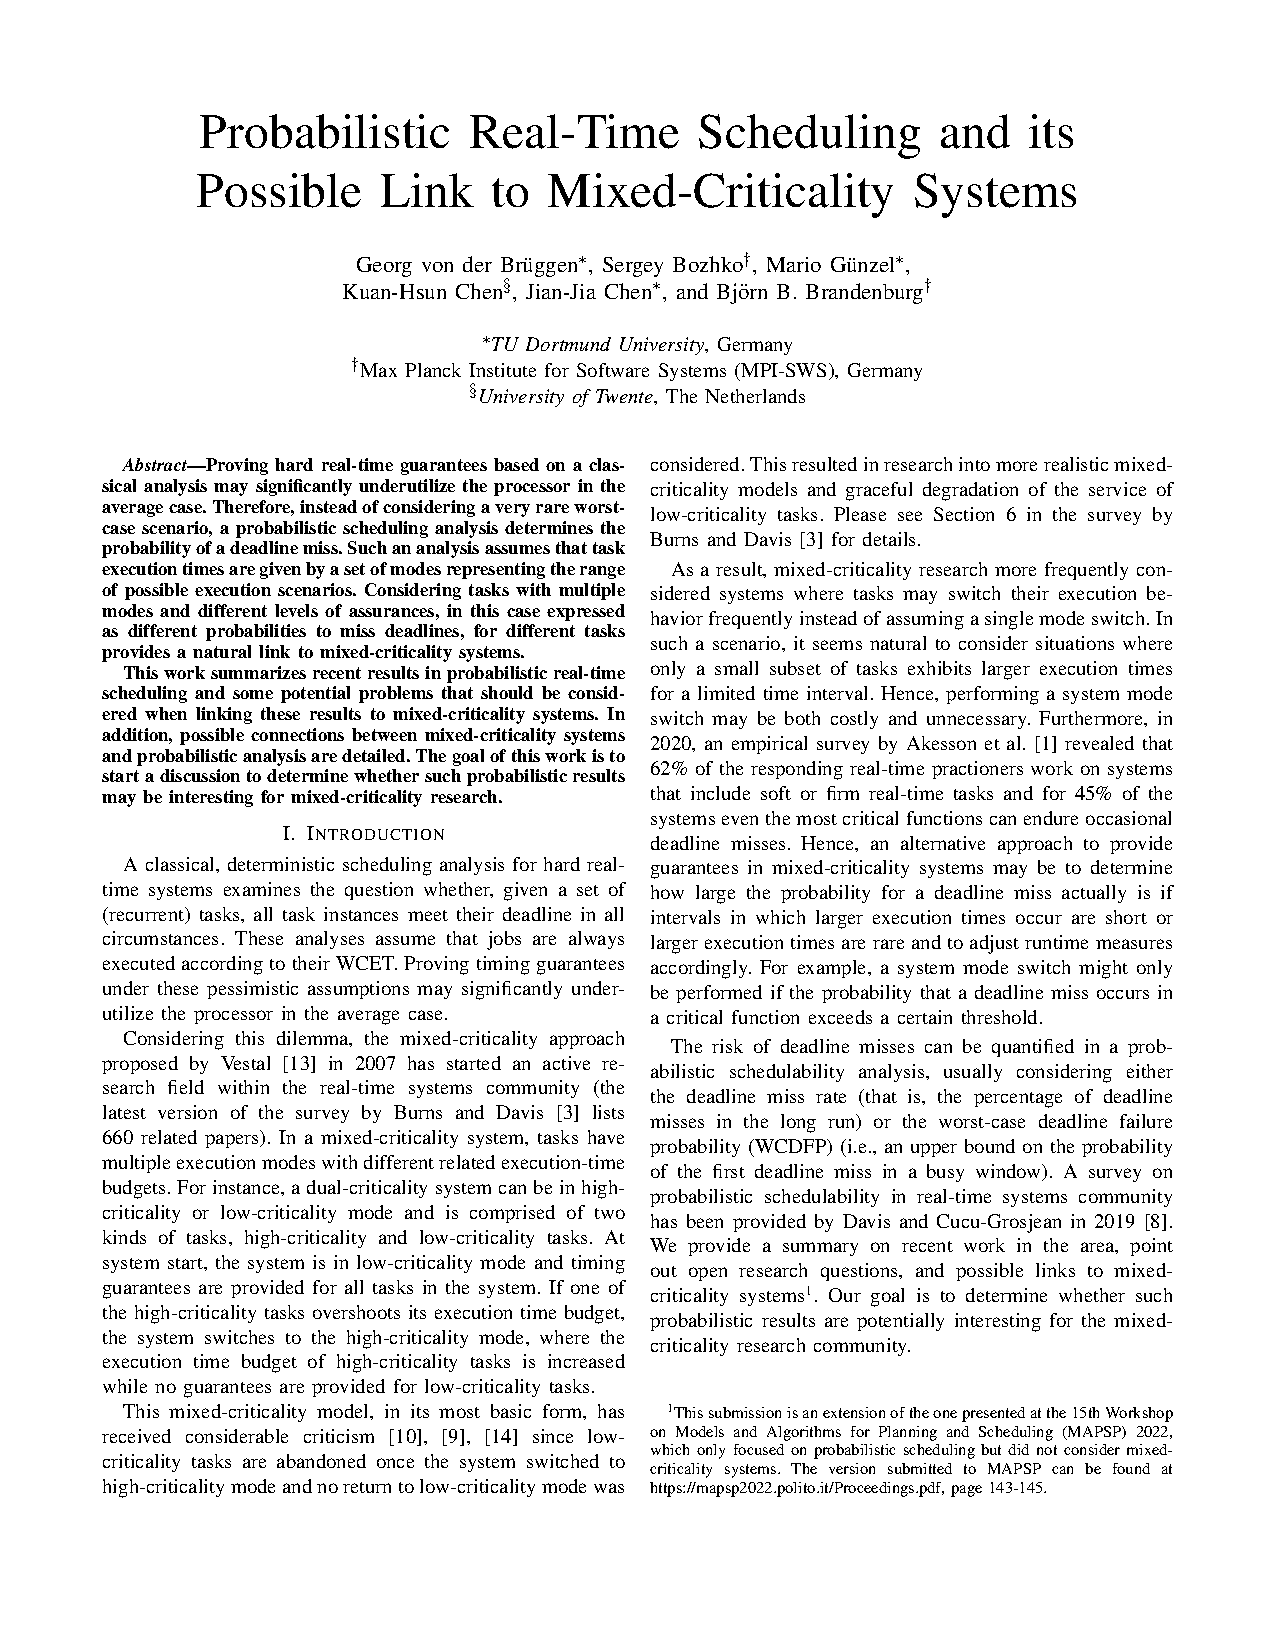
\includepdf[pages=-]{papers/9978.pdf}

\addcontentsline{toc}{subsection}{Mixed-Criticality Scheduling for Parallel Real-Time Tasks with Resource Reclamation}
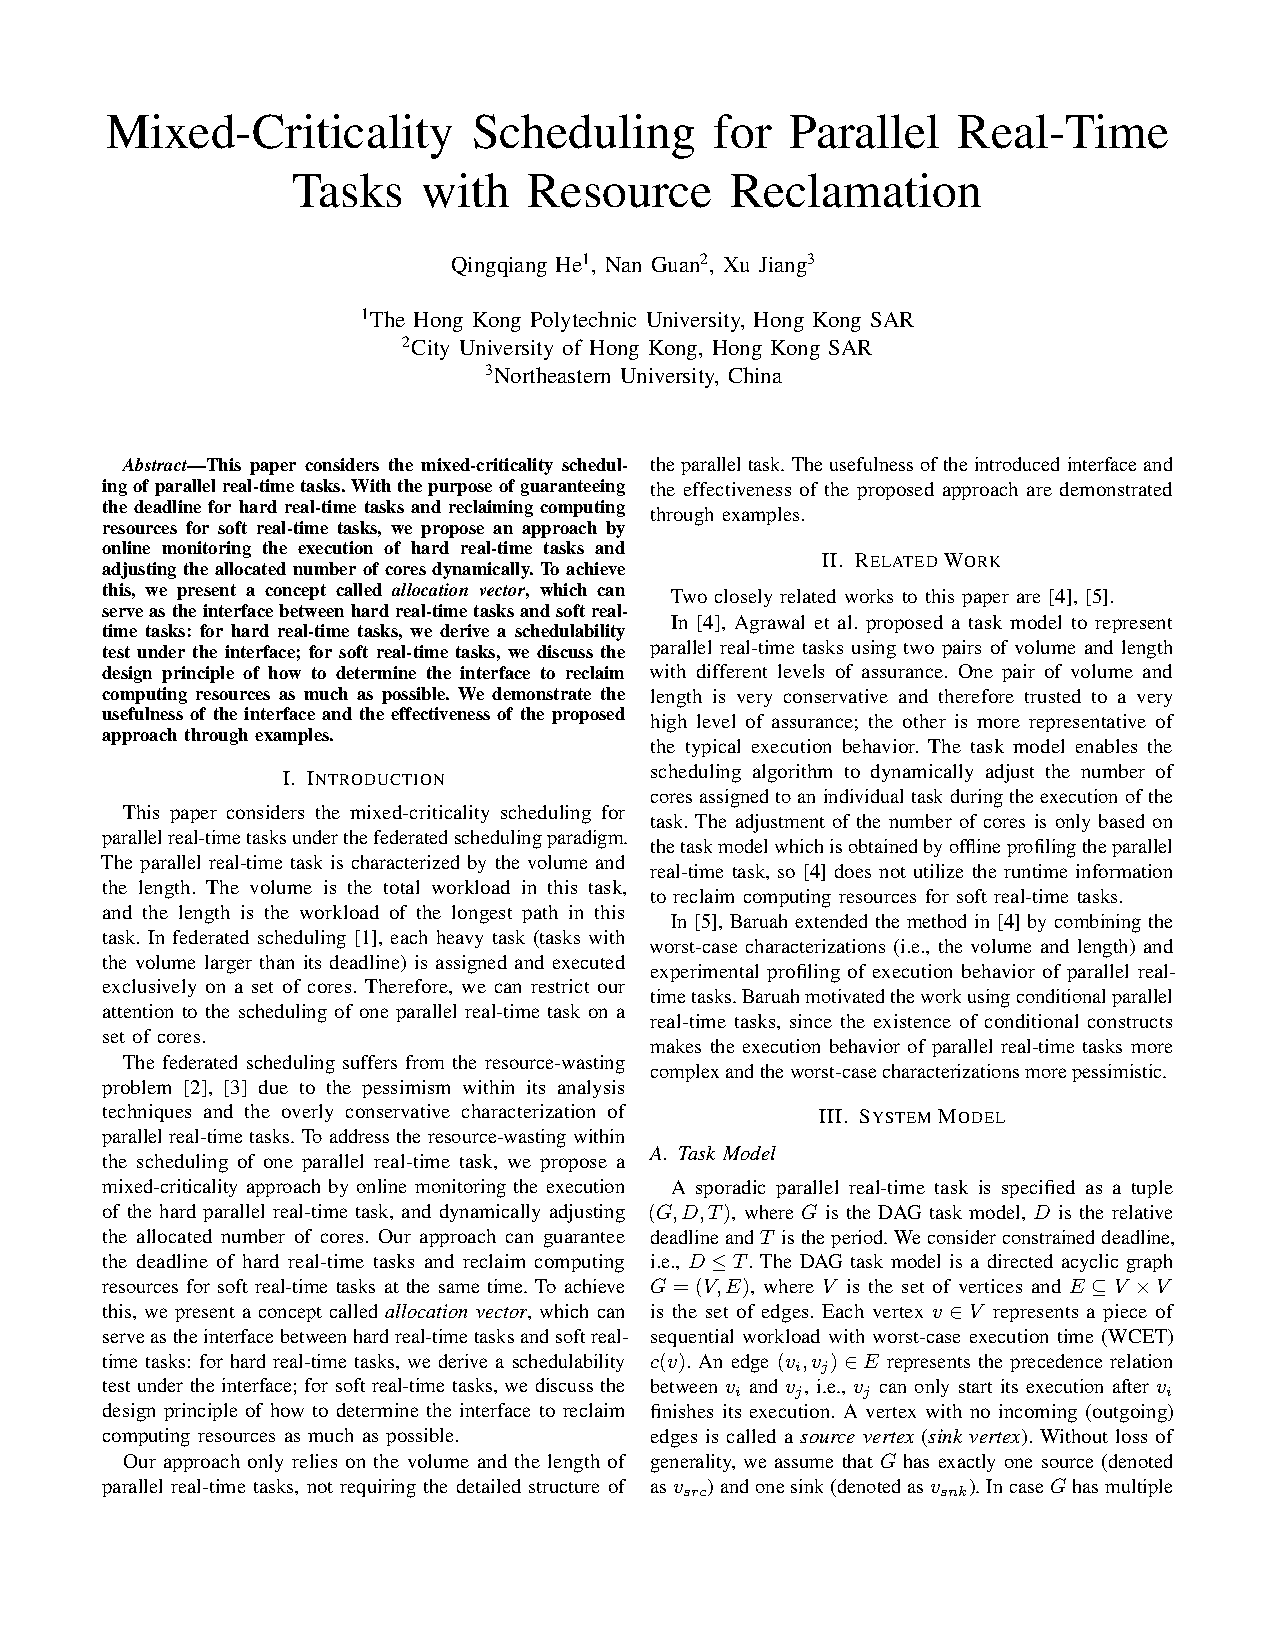
\includepdf[pages=-]{papers/1935.pdf}

\addcontentsline{toc}{subsection}{A Secure Resilient Real-Time Recovery Model, Scheduler, and Analysis}
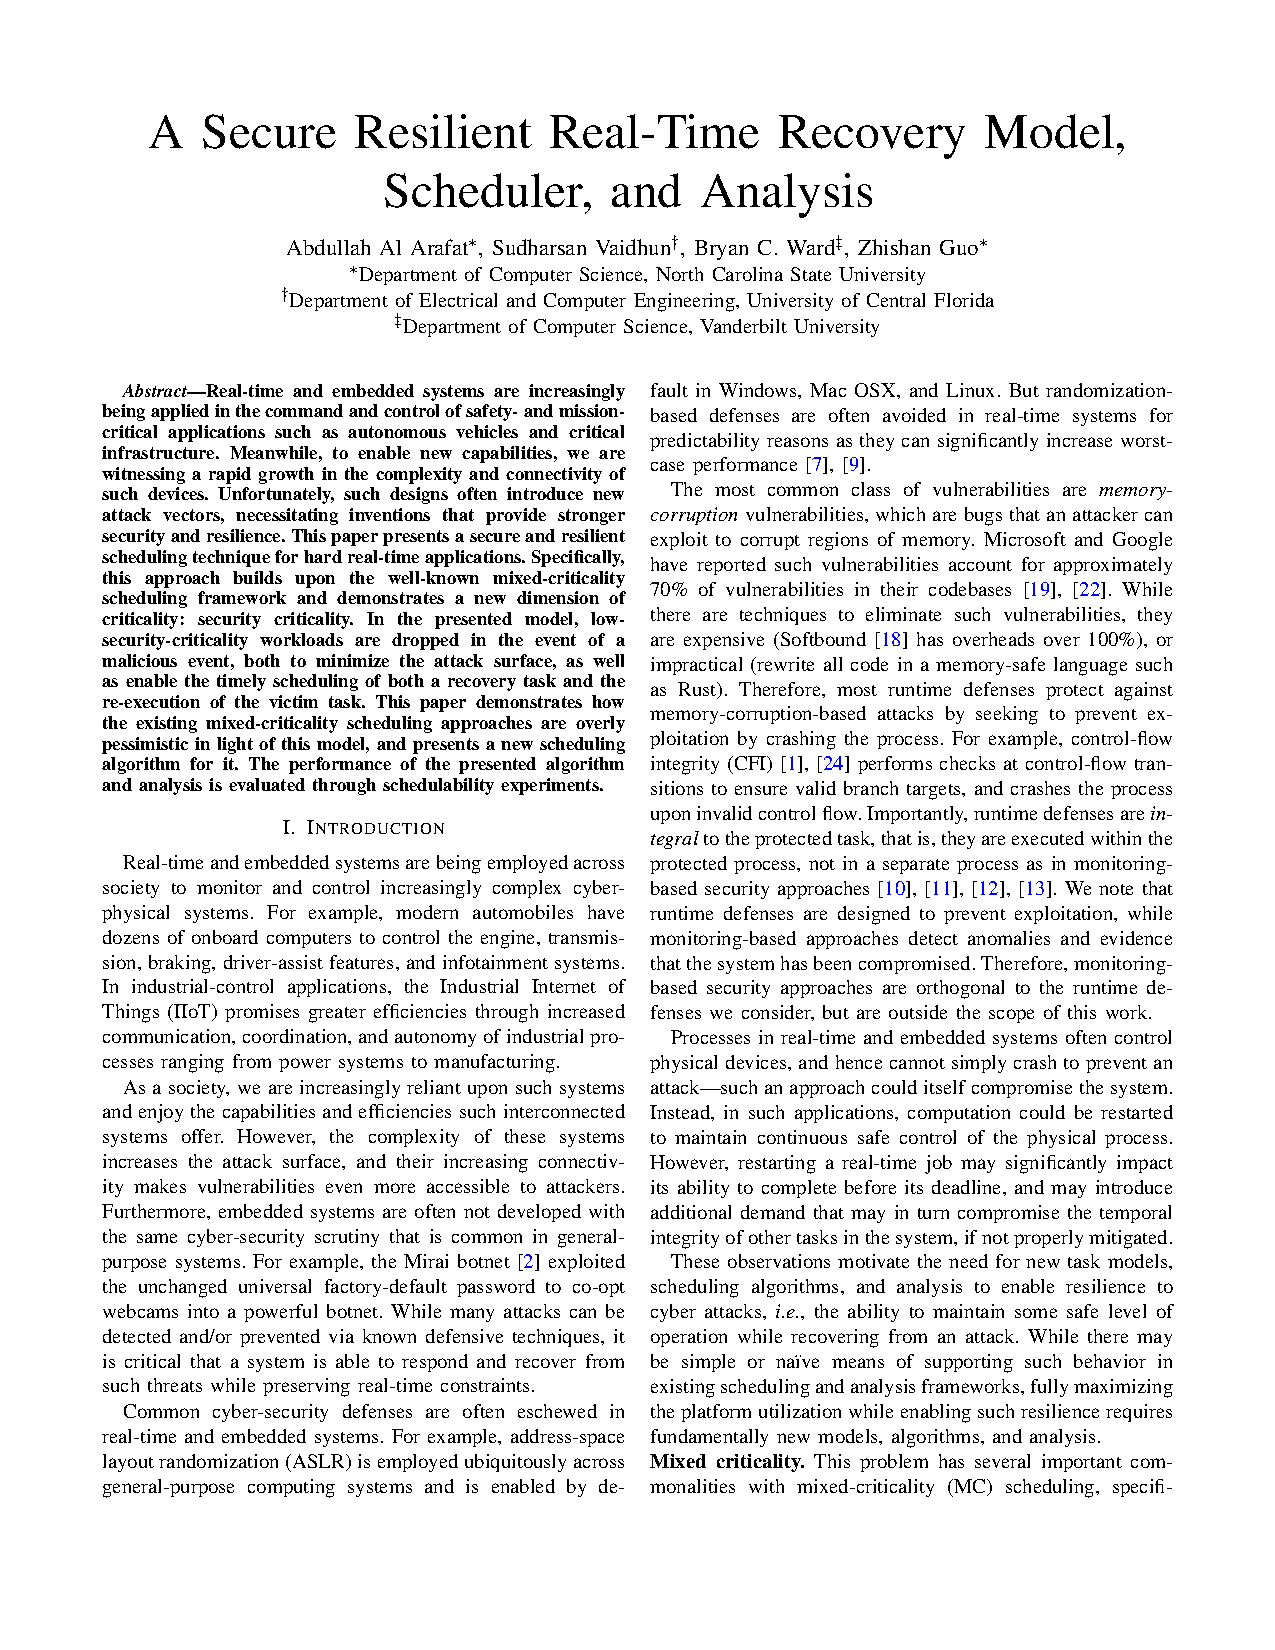
\includepdf[pages=-]{papers/2884.pdf}

\addcontentsline{toc}{subsection}{Mixed-Criticality Wireless Communication for Robot Swarms}
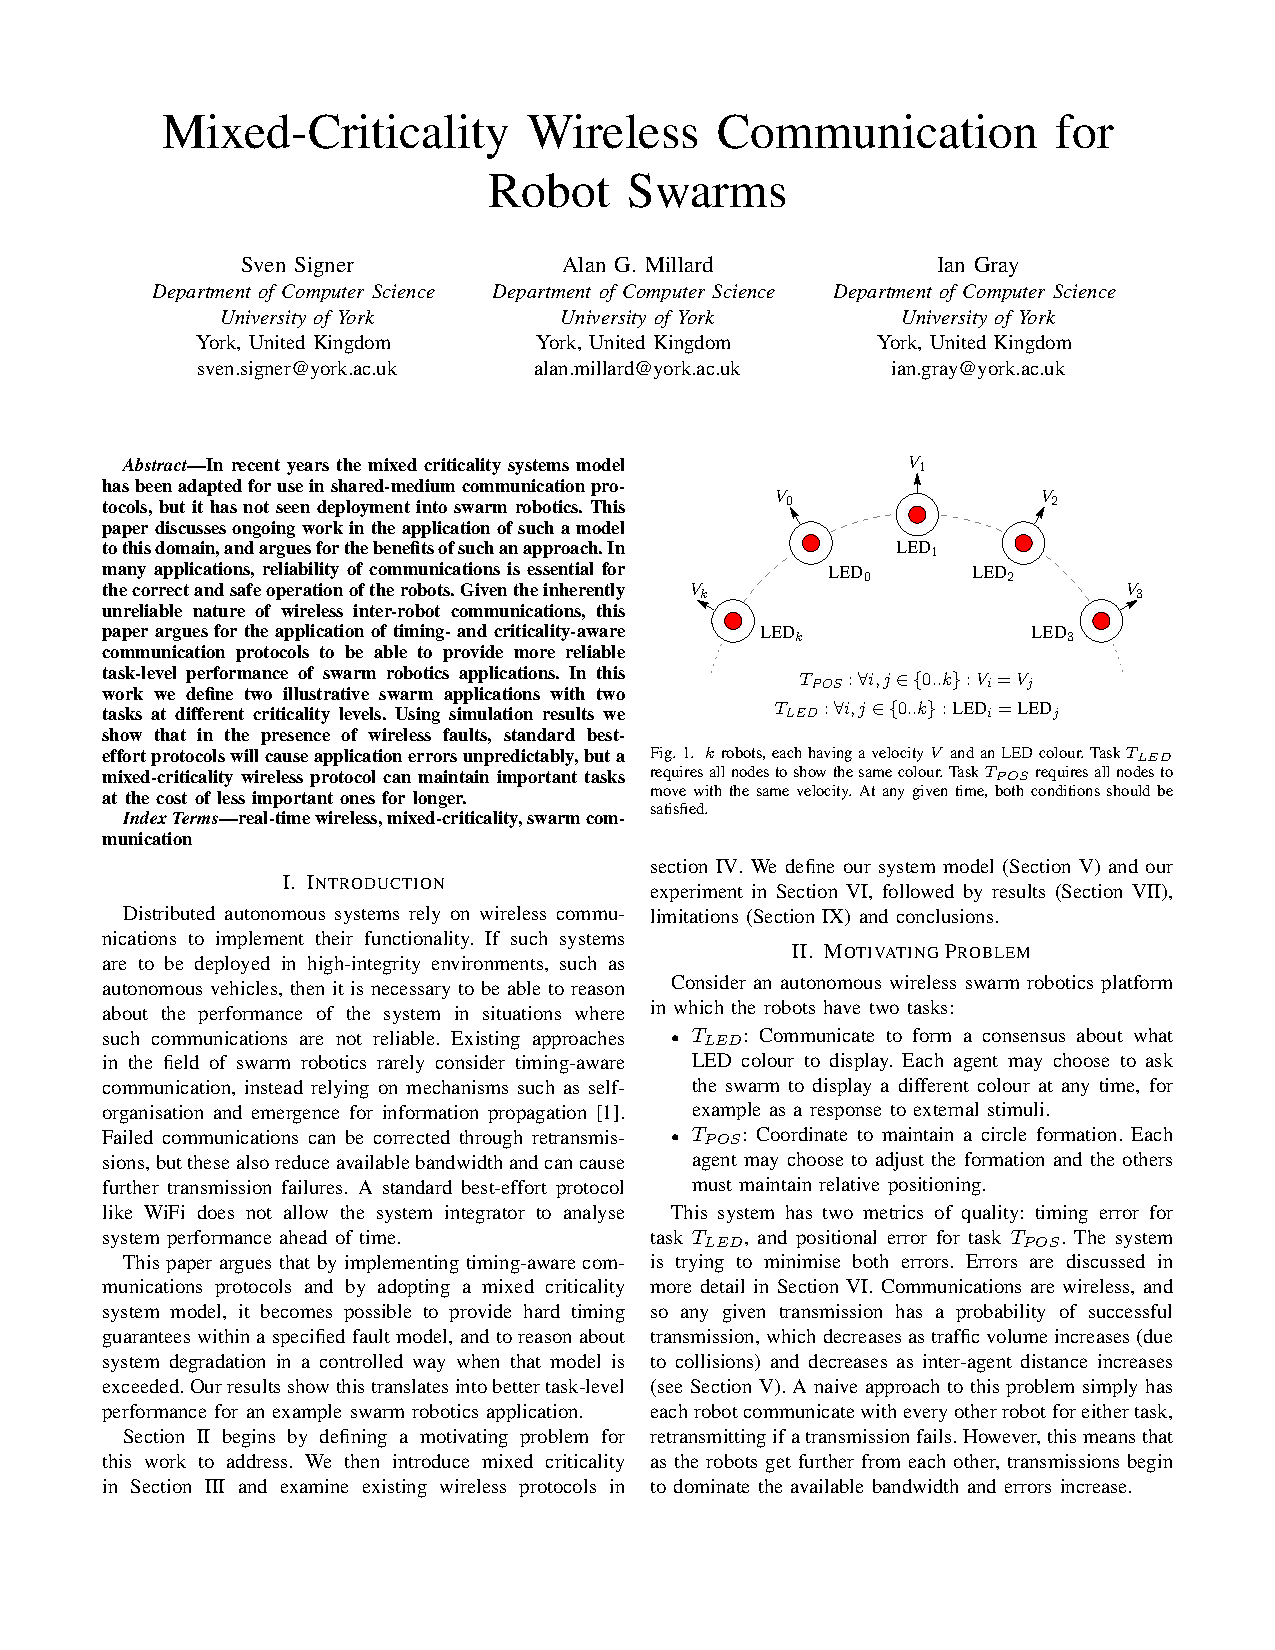
\includepdf[pages=-]{papers/4220.pdf}

\addcontentsline{toc}{subsection}{Precise Scheduling Mixed-Criticality Gang Tasks with Reserved Processors}
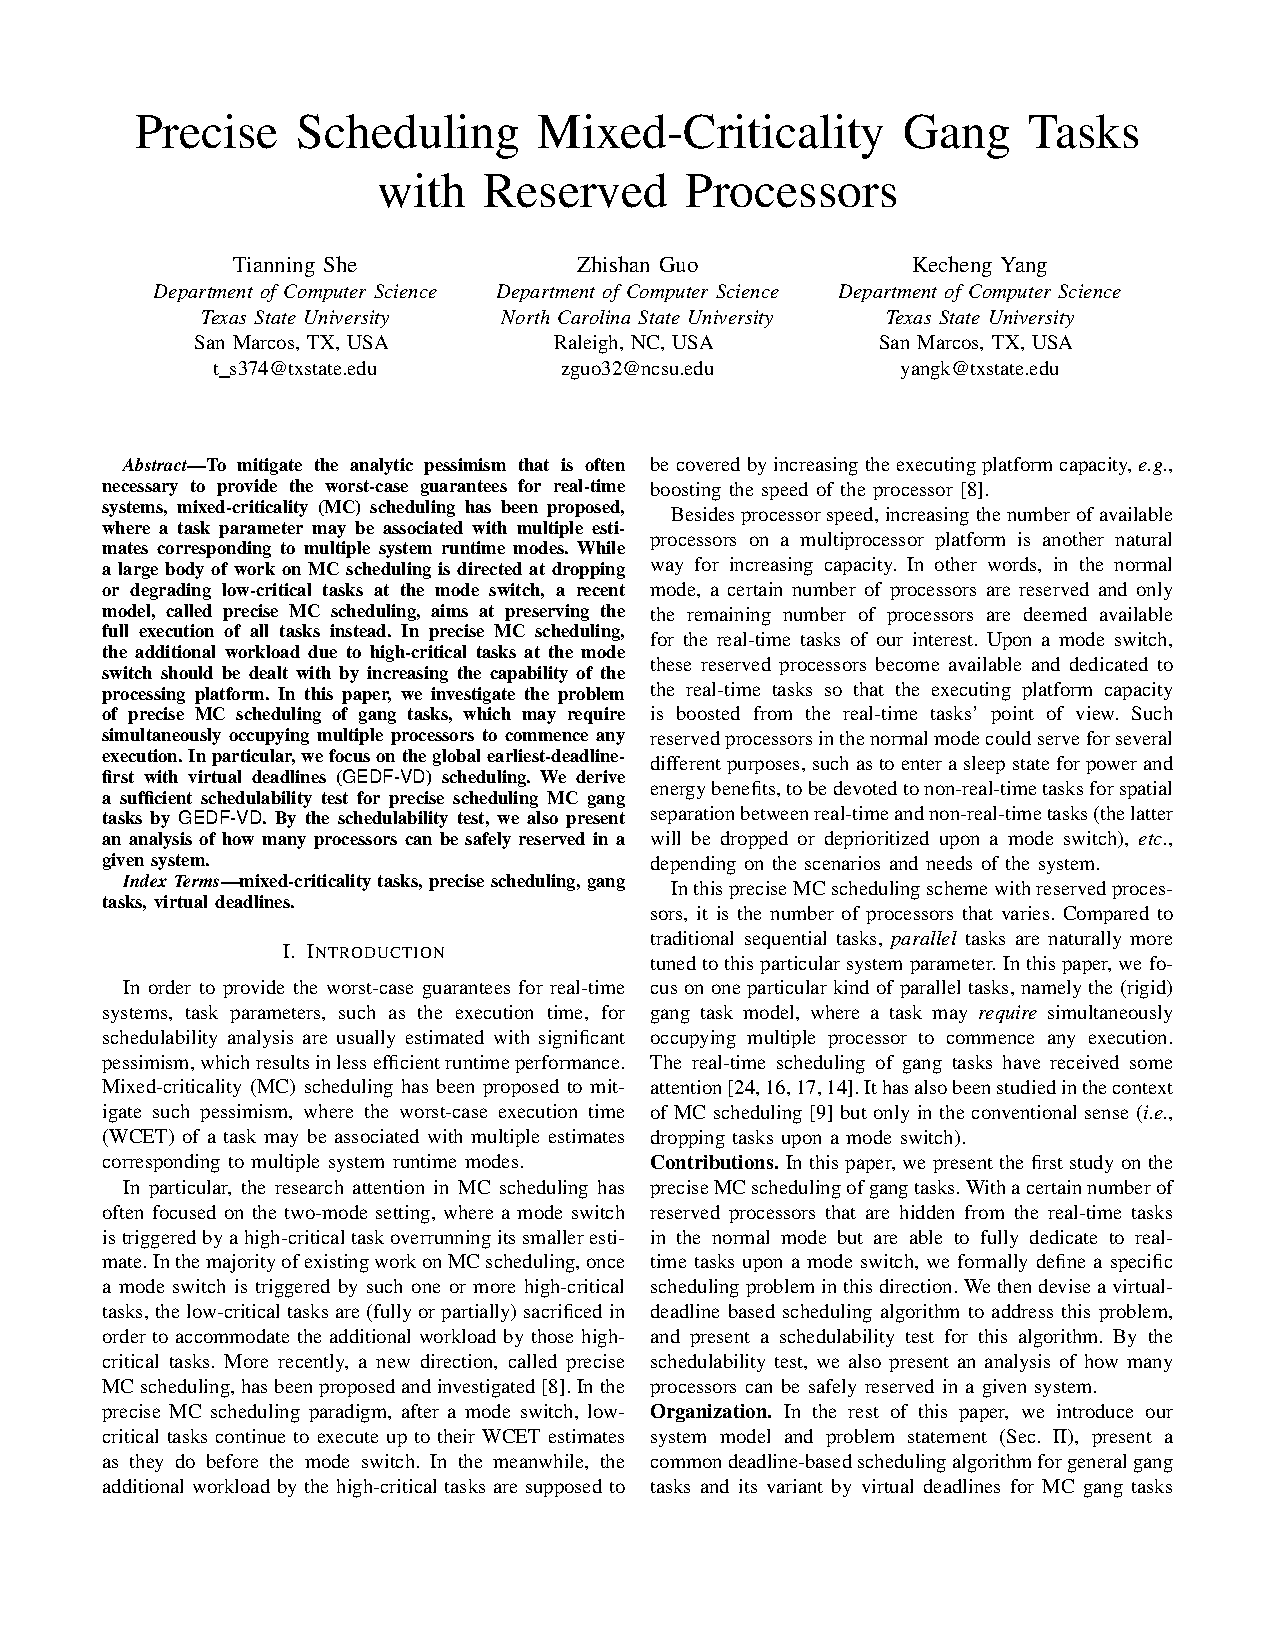
\includepdf[pages=-]{papers/6254.pdf}

\addcontentsline{toc}{subsection}{A High-Resilience Imprecise Computing Architecture for Mixed-Criticality Systems}
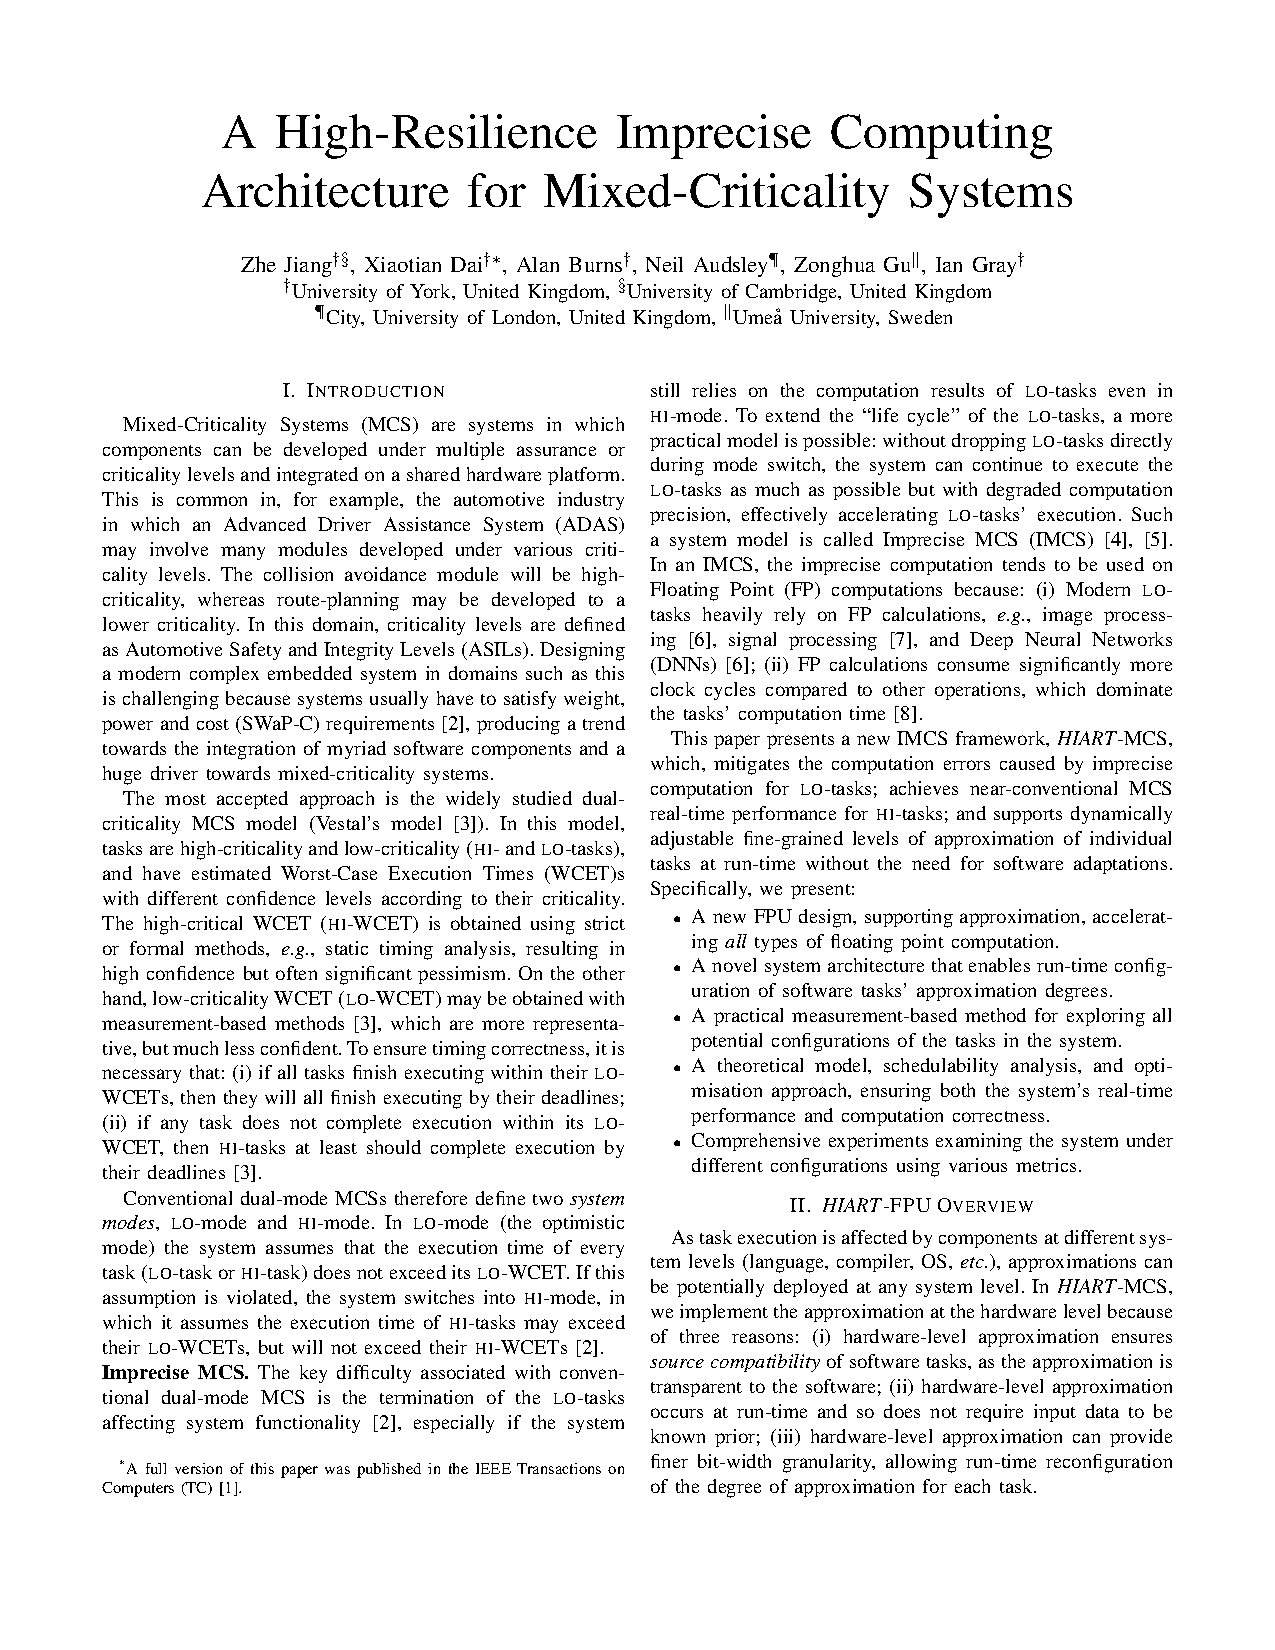
\includepdf[pages=-]{papers/3961.pdf}

\addcontentsline{toc}{subsection}{Computing the Execution Probability of Jobs with Replication in Mixed-Criticality Schedules}
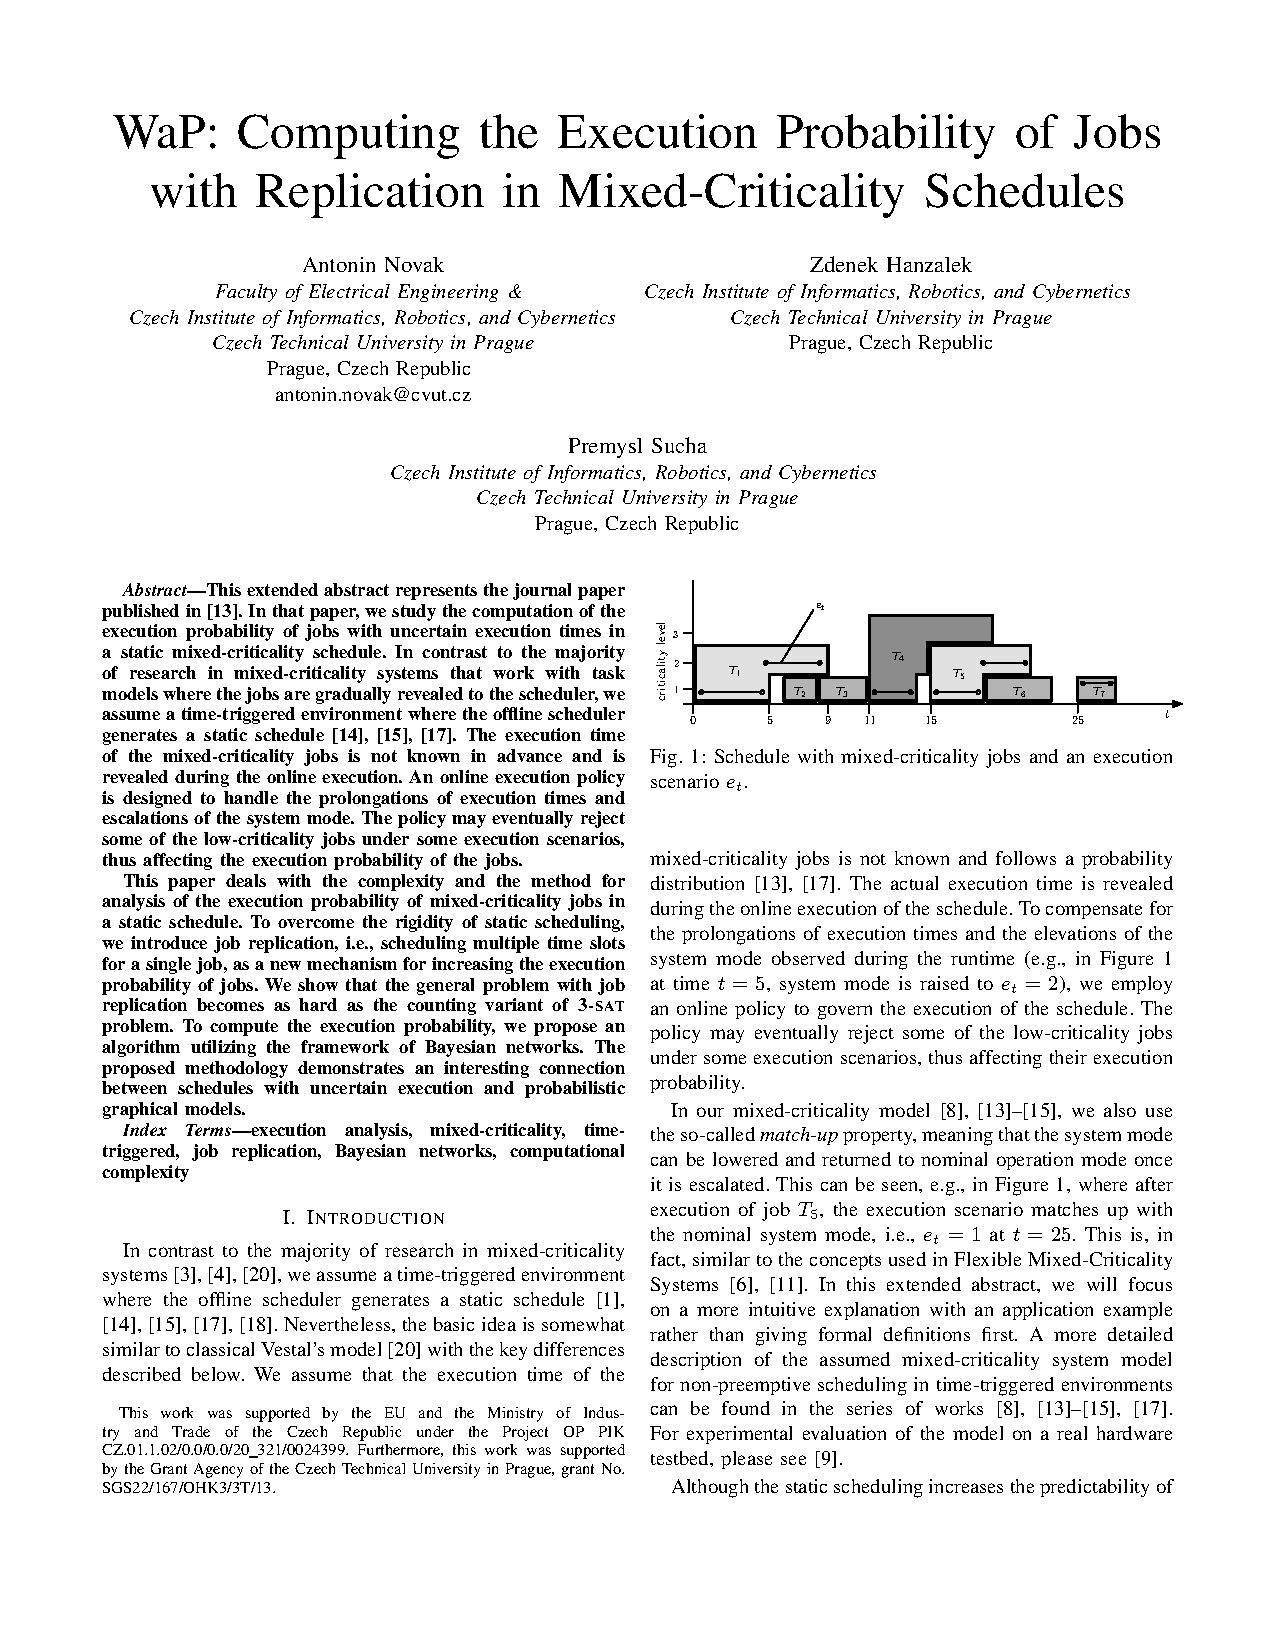
\includepdf[pages=-]{papers/5290.pdf}

\addcontentsline{toc}{subsection}{Bridging the Pragmatic Gaps for Mixed-Criticality
Systems in the Automotive Industry}
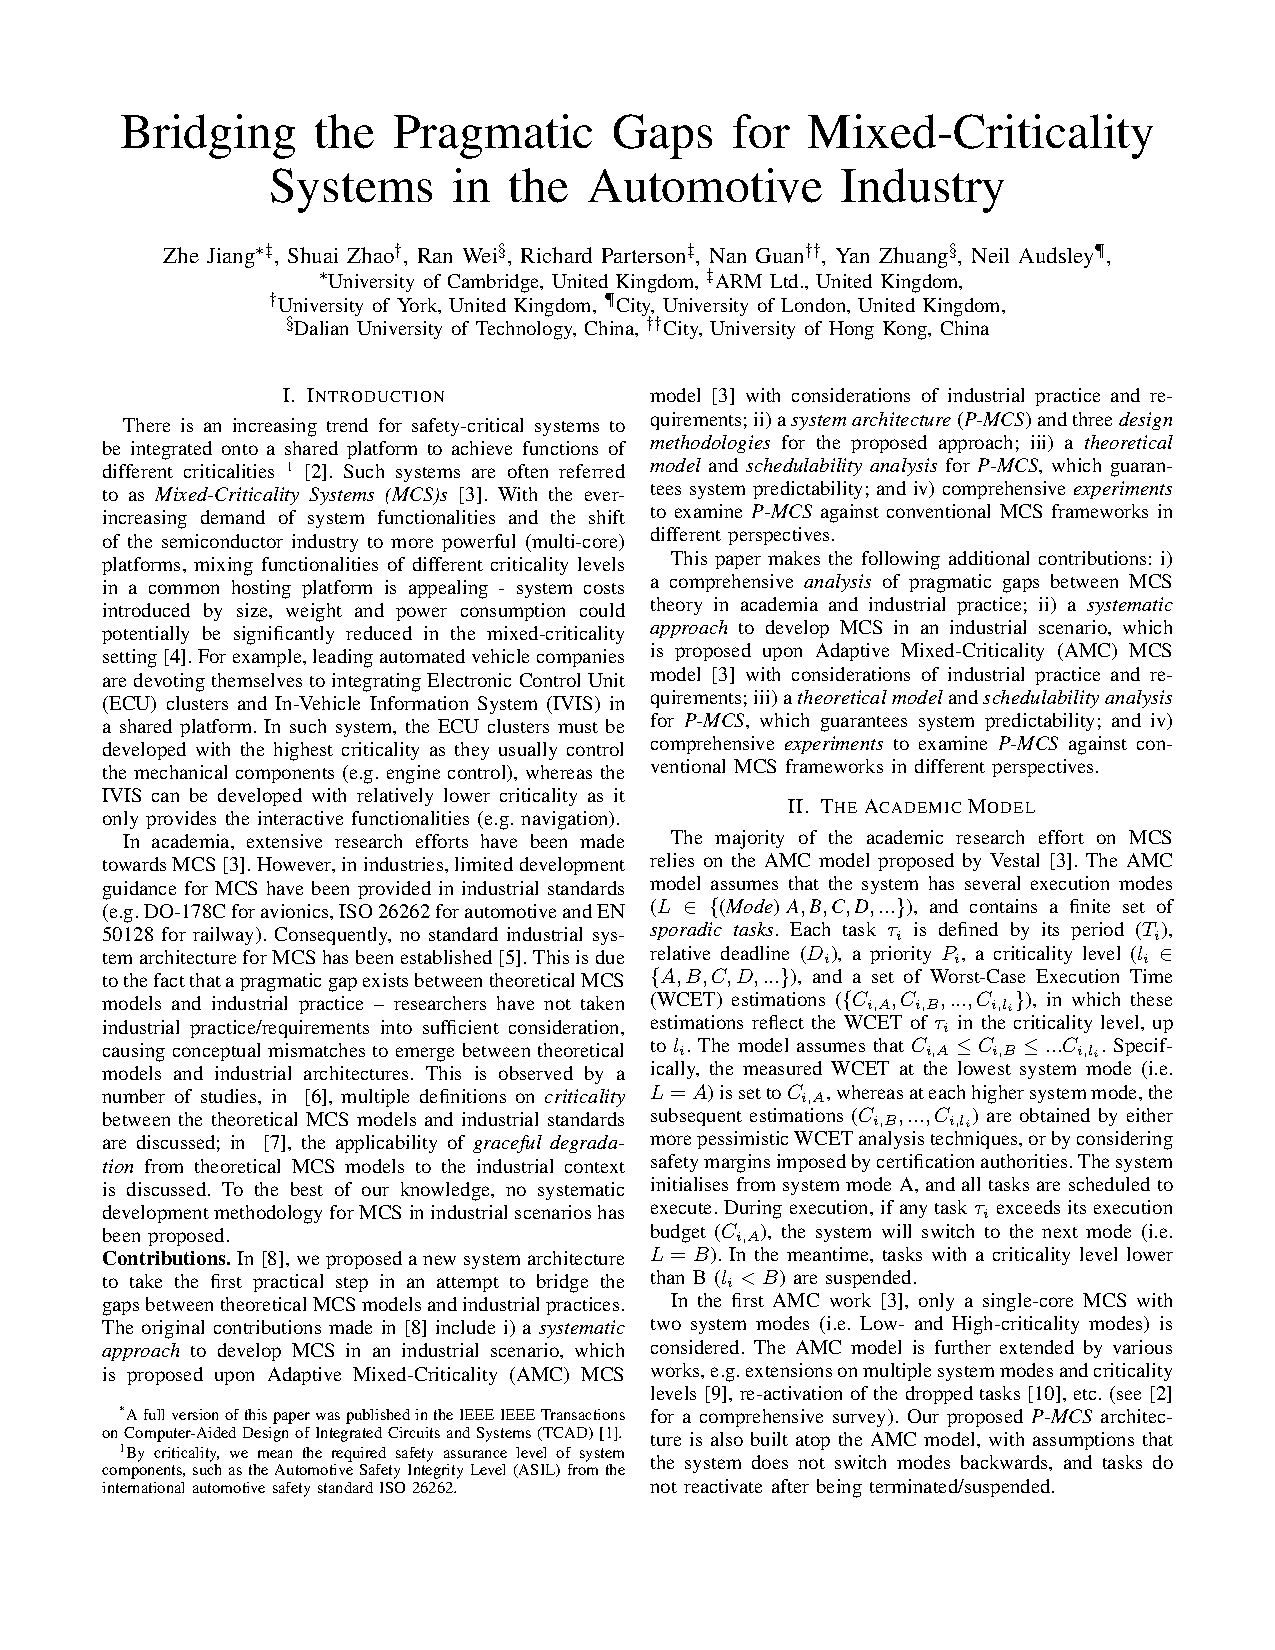
\includepdf[pages=-]{papers/8669.pdf}

\clearpage

\end{document}
